\documentclass[english,11pt,twoside,a4paper]{article}
\usepackage[left=2cm,top=1cm,right=2cm,nohead,nofoot]{geometry}
\usepackage[utf8]{inputenc}
\usepackage{hyperref}
\usepackage{amssymb}
\usepackage{graphicx}
\usepackage{titling}
\newcommand{\subtitle}[1]{%
  \posttitle{%
    \par\end{center}
    \begin{center}\large#1\end{center}
    \vskip0.5em}%
}

\begin{document}
\author{
  Niemistö, Jesse
  \and
  Muona, Leo
  \and
  Hilden, Matias
}
\title{Raspberry Pi robot}
\subtitle{Intelligent Embedded Systems - Final report}

\maketitle

\tableofcontents

\section{Introduction}

This is a final report for the course Intelligent Embedded System (id 582711) at the CS Department of the University of Helsinki. This course was held at during Spring term 2014, third period. The course is a self-study course that consists of an embedded systems project. For our project we chose to build a Raspberry Pi robot, which utilizes Pi's camera module, audio output and electric DC motors.

Raspberry Pi is a cheap arm-computer that was originally created for the purpose to help more people to get into programming. We chose to use this one-chip-computer for our project because it runs on Linux (among other operating systems), it has a camera module available, it has GPIO pins for controlling a motor control chip, and all of our team members already had one lying around.

This document includes our project idea, requirements and initial design for the robot, implementation of the robot, evaluation of our project, and a summary of lessons learned. This is the tale of our awesome little raspi robot.

\section{The idea}

We got our initial idea from the video game Portal by Valve Corp. In the game, there were these "cute" robot turrets that recognized movement, talked to the source of the movement and shot them. So our initial idea was to create a robot similar to these turrets, so that we will use Raspberry Pi's camera module to recognize movement, target the movement source, and play a random audio clip to greet the source of the movement.

Our initial idea had two DC motors to control the turret's movement and a laser- or LED-pointer to point the target. However this idea evolved during the project just to use one motor and only turn the camera towards the movement source.

\section{Requirements and initial design}

At the start of our project we wrote our requirements and then initial design. The design consists more on actual planning of hardware part, than the code to be created. This section can be divided into five parts: required features, audio system design, camera design, motor control system design, and software design.

\subsection{Required features}

These were our required features at the start of our project when designing the robot:

\begin{itemize}
  \item Horizontal and vertical rotational movement.
  \item WAV (or ogg) audio playback.
  \item Motion detection based on frame difference algorithm.
  \item Aiming at detected movement.
  \item Remote control.
  \item Works on top of Linux.
\end{itemize}

We used these features a guideline for our project design. At this stage it is good to mention that some of these features were modified during the project.

\subsection{Audio design}
\label{sec:audio_design}

For audio we used the 3.5mm jack audio output connector on the raspberry pi with our self-built audio amplifier, which is connected to a single speaker. The single speaker can only output mono audio, but this won't matter since audio contains only speaking. The used speaker was small and low powered. We also made a simple audio jack connector. This was made with a bought 3.5mm mono jack connector, which was soldered to ground and audio.

\begin{figure}
  \begin{center}
    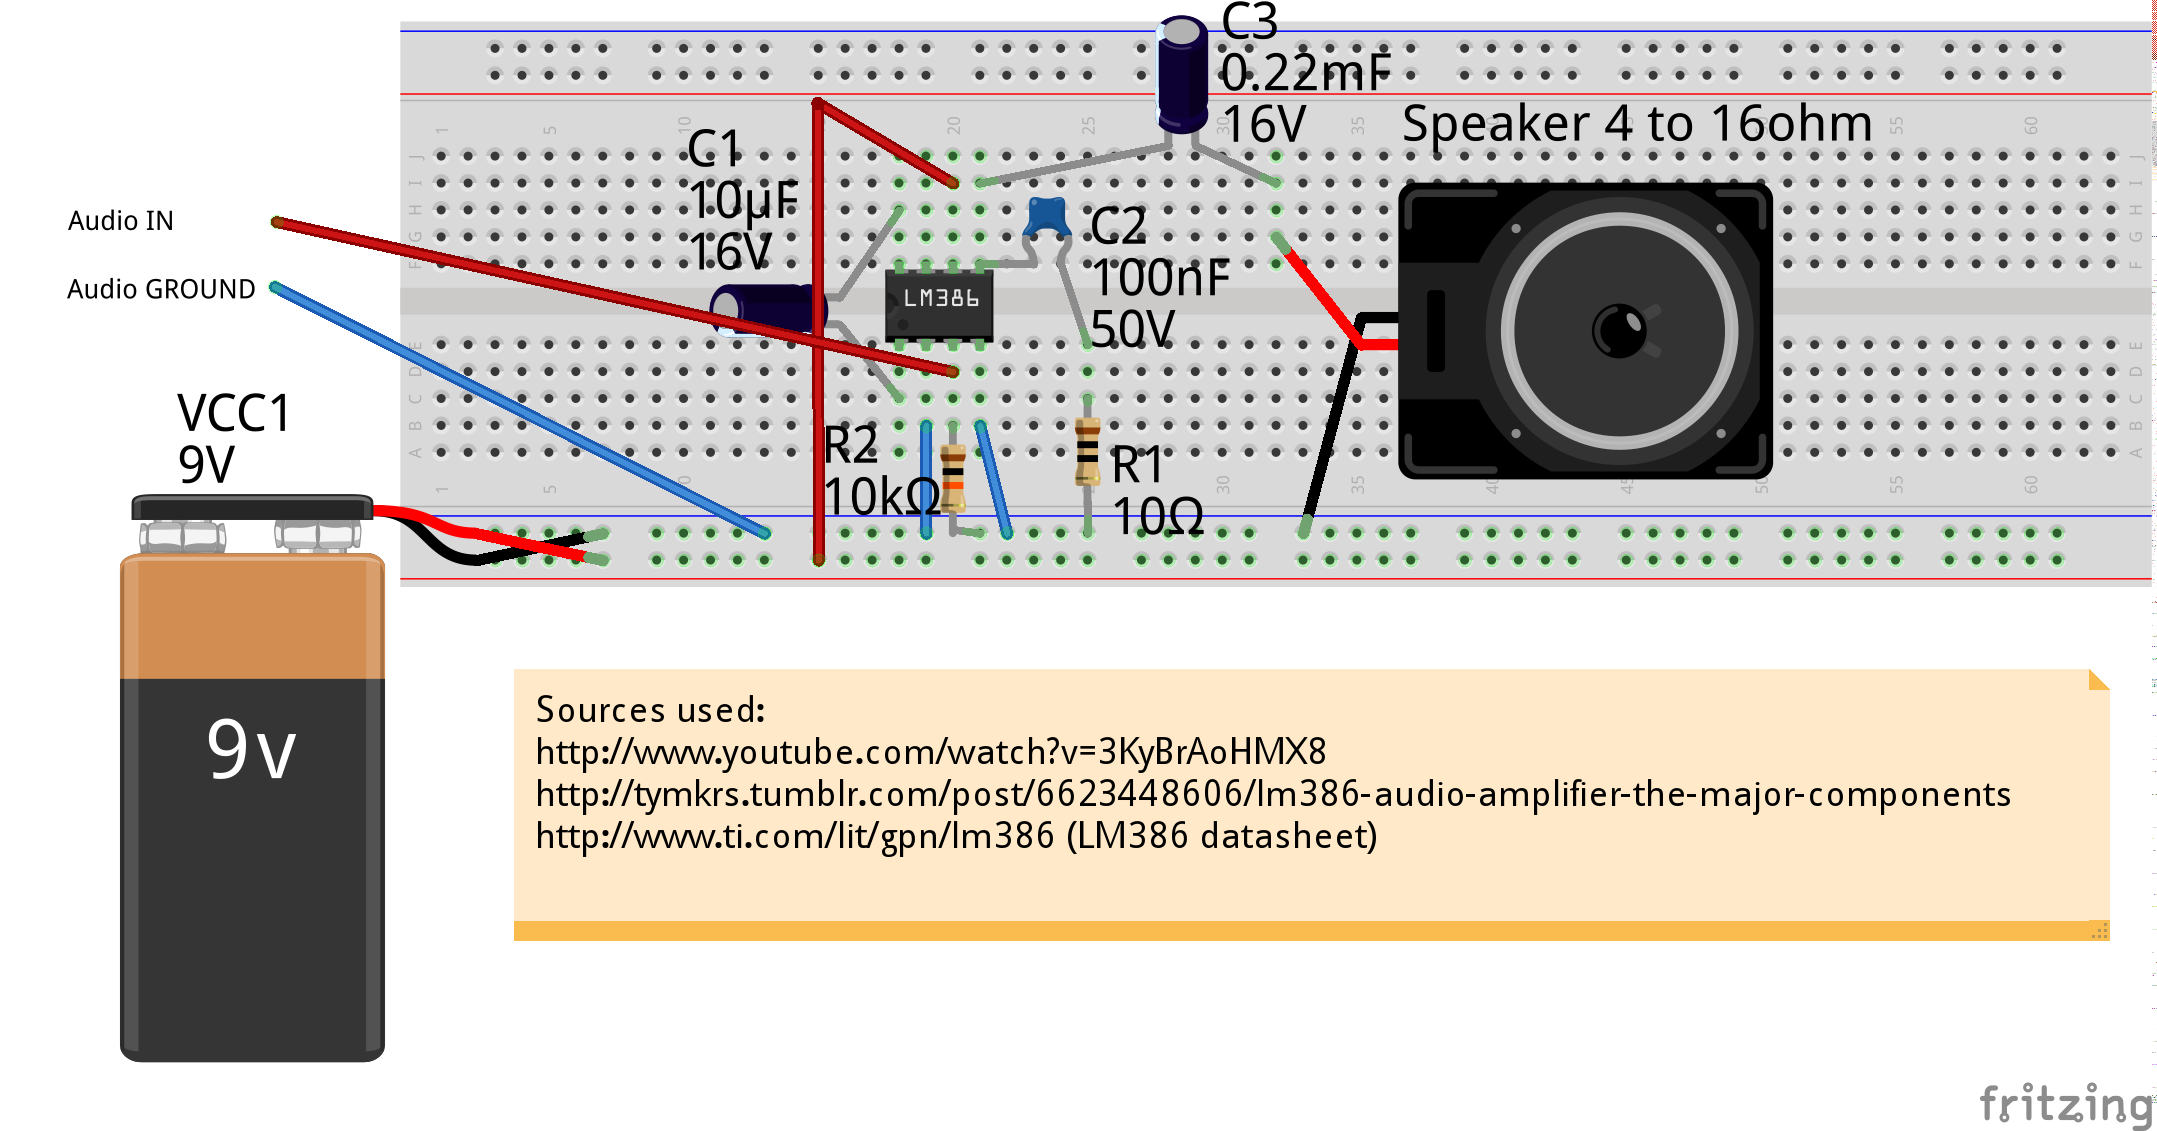
\includegraphics[scale=0.75]{audio_amplifier_lm386_bb.png}
    \caption{Breadboard view for the audio amplifier.}
  \end{center}
  \label{lm386_bb}
\end{figure}

In the heart of the audio amplifier stands the LM386 circuit, which is a "Low Voltage Audio Power Amplifier" and was more than enough for our use case. The figure in~\ref{lm386_bb} shows the breadboard view that we used used for the audio amplifier. The build is same to that what is shown on the LM386 datasheet, "amplifier with Gain = 200".

\begin{itemize}
  \item Between PINs 1 and 8 is a 10uF capacitor, which causes a gain on 200. In desibels this is around 20.
  \item PIN 2 is places to ground.
  \item PIN 3 takes the audio input, and is connected to ground through 10k ohm resistor.
  \item PIN 4 is placed to ground.
  \item PIN 5 is the amplified audio output.
  \item PIN 6 takes power
  \item PIN 7 is bybassed, doesn't take connection.
\end{itemize}

\subsection{Camera design}

We decided to use a simple plug-in Raspberry Pi camera module, which we will use to take pictures that we compare to previous ones to detect movement. Since Raspberry Pi has a ready-to-use socket for camera cable, no extra cables or power supplies are needed. To use the camera we will use \href{https://github.com/raspberrypi/userland}{Pi's Userland code}, that comes with raspistill-program which we can use to take still pictures.

\subsection{Motor control design}

To control the motors, we planned our design around L293D motor control chip, which is cheap and easily available. Our design consisted of two motors, one to turn the camera horizontally and one to turn the camera vertically. This design used two L293D chips, one for each motor.

\begin{figure}
  \begin{center}
    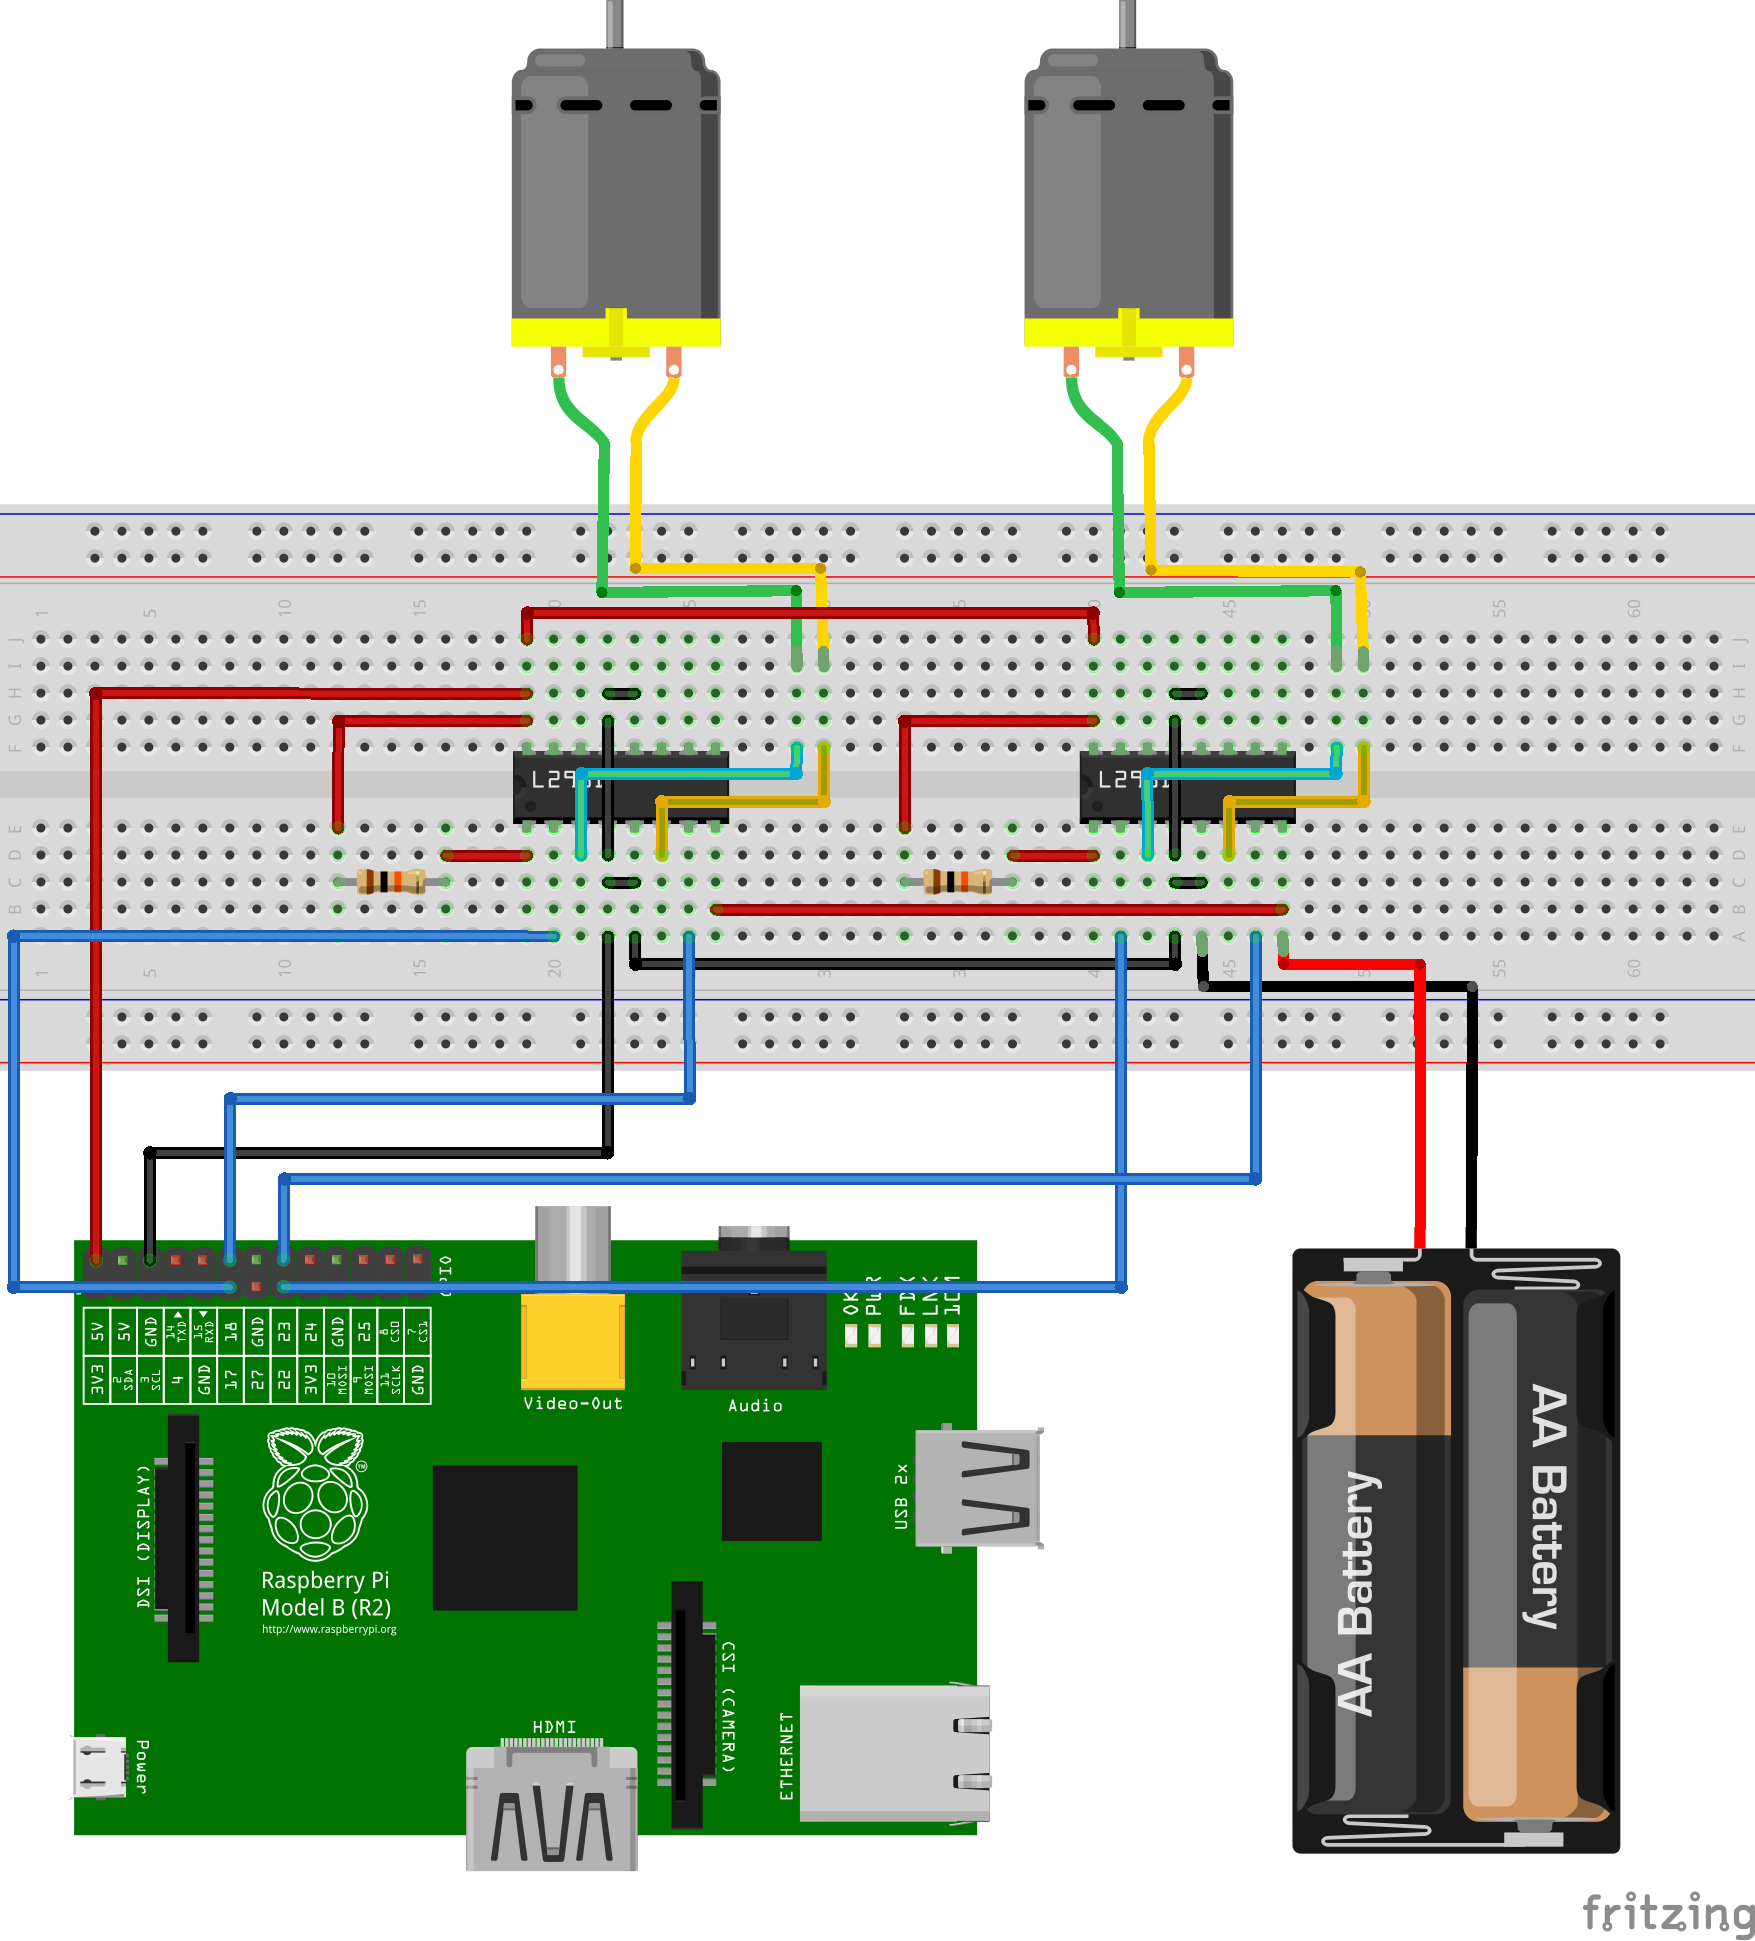
\includegraphics[scale=0.75]{motor_controllers_l293d_bb.png}
    \caption{Motor controllers design in breadboard view.}
  \end{center}
  \label{l293d_bb_design}
\end{figure}

Figure \ref{l293d_bb_design} shows how the chips would be connected into the Raspberry Pi. Design uses GPIO pins 17 and 18 to control the first motor and pins 22 and 23 to control the second motor. The two AA batteries will supply power for both of the motors, and Raspberry Pi will supply power for the motor control chips.

\subsection{Software design}

Our project requires software for three main things: camera control, audio control and motor control. Even though we use a ready-to-use software to take pictures with the camera, we need to write our own software for image analysis, that is used to detect movement in the camera. We will write our own audio playback code against pulseaudio sound server. As for sound files, we are planning to use .ogg files. For the motor controlling we plan to use either direct /dev/mem code, or an additional WiringPi gpio library to control the GPIO pins.

We will also write other code, like the logical code for the whole software, and a remote control code for testing purposes. And hopefully we don't need to write multiple hacks.

\section{Implementation}

\subsection{Audio}

The implementation of the audio amplifier required bying the parts and assembling them. There weren't really any problems with this, and everything worked as was planned. Refer to chapter~\ref{sec:audio_design} for what was the plan.

The speaker didn't require any assembling but was simply connected to the audio amplifier. For the case of our speaker we used a beer can. Twas used for flavor.

\section{Evaluation}

\subsection{Audio}

Audio amplifier, when connected to the speaker had suprisingly good sound and volume. Actually we had to drop to volume to one fourth of what was the full volume not to break our ears. The speaker in a can outputted a good and clear sound, better than any of us could have hoped for.

However, when audio jack is not connected, and even sometimes when connected, the audio amplifier and speaker takes audible interference. A high-piched noise that eats into your mind. There were a few workarounds, that mostly was duct taping the wires together which acted as a shield for the wires.

\section{Summary}

TODO

\end{document}
